\documentclass[12pt, spanish]{beamer}
\usepackage[spanish]{babel}

\usetheme{metropolis}
% \setbeamertemplate{itemize items}[default]
% \setbeamertemplate{enumerate items}[circle]


% --- TITULO --- 
\title{Mejora de un Sistema de Auto-escalado para Sistemas Distribuidos}

\subtitle{Trabajo de Fin de Grado\\{\small Grado de Ingeniería Informática}}

\author[CMA]{\textit{Autor:} Miguel Alonso, Carlos\\\textit{Tutor:} Rampérez Martín, Victor}

\institute{ETSIINF - Universidad Politécnica de Madrid}

\date{Febrero - 2022}
% --- TITULO ---


\begin{document}


%%%%%%%%%%%%%%%%%%%%%%%%%%%%%%%%%%%%%%%%%%%%%%%%%%%%%%%%%%%%%%%%%%%%%%%%%%%%%%%%

\begin{frame}%{Portada}
    \titlepage
\end{frame}

%%%%%%%%%%%%%%%%%%%%%%%%%%%%%%%%%%%%%%%%%%%%%%%%%%%%%%%%%%%%%%%%%%%%%%%%%%%%%%%%

\begin{frame}{Indice}
    \begin{enumerate}
        \item Motivación del proyecto\vspace{0.1cm}
        \item Objetivos\vspace{0.1cm}
        \item Estado del Arte\vspace{0.1cm}
        \item Diseño e implementación de un generador de cargas de trabajo para sistemas pub/sub basados en contenido\vspace{0.1cm}
        \item Pruebas de rendimiento\vspace{0.1cm}
        \item Implementación de los modelos predictivos\vspace{0.1cm}
        \item Resultados y Conclusiones\vspace{0.1cm}
        \item Trabajo futuro
    \end{enumerate}
\end{frame}

%%%%%%%%%%%%%%%%%%%%%%%%%%%%%%%%%%%%%%%%%%%%%%%%%%%%%%%%%%%%%%%%%%%%%%%%%%%%%%%%

\begin{frame}{Motivación del proyecto}
    \begin{itemize}
        \item Digitalización de la vida diaria\vspace{0.1cm}
        \item Cloud Computing $\implies$ elasticidad \& \textit{pay-as-you-go}\vspace{0.1cm}
        \item Sistemas publicador/subscriptor auto-escalables\vspace{0.1cm}
        \item Carga de trabajo de contexto real\vspace{0.1cm}
        \item E-SilboPS
    \end{itemize}
\end{frame}

%%%%%%%%%%%%%%%%%%%%%%%%%%%%%%%%%%%%%%%%%%%%%%%%%%%%%%%%%%%%%%%%%%%%%%%%%%%%%%%%

\begin{frame}{Objetivos}
    \begin{enumerate}
        \item Estudio del estado del arte\vspace{0.2cm}
        \item Estudio de cargas de trabajo de contexto real para sistemas pub/sub basados en contenido\vspace{0.2cm}
        \item Diseño e implementación de pruebas de rendimiento que utilicen esta carga\vspace{0.2cm}
        \item Diseño e implementación de modelos predictivos sobre el rendimiento\vspace{0.2cm}
    \end{enumerate}
\end{frame}

%%%%%%%%%%%%%%%%%%%%%%%%%%%%%%%%%%%%%%%%%%%%%%%%%%%%%%%%%%%%%%%%%%%%%%%%%%%%%%%%

\begin{frame}%{Estado del Arte}
    \begin{center}
        {\Large\textbf{Estado del Arte}}
    \end{center}
\end{frame}

\begin{frame}{Estado del Arte - Sistemas p/s} % Fundamentos teóricos => Estado del Arte resumido
    \centering

    \begin{figure}
        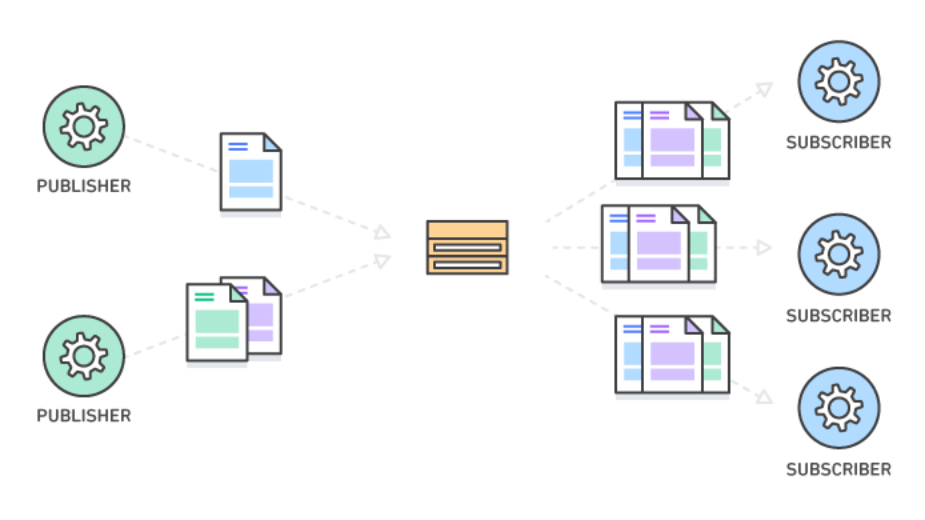
\includegraphics[width=0.8\textwidth]{images/pubsub-diagram.png}
    \end{figure}
    \textbf{Paradigma publicador/subscriptor}
    
\end{frame}

\begin{frame}{Estado del Arte - Escasez de cargas de trabajo reales}
    Escasez de cargas de trabajo originadas de contexto real\vspace{1cm}
    
    Problemas...
    \begin{itemize}
        \item Privacidad de datos (usuarios y empresas)
        \item Intereses de los usuarios en las subscripciones\vspace{1cm}
    \end{itemize}
    
    \textit{Cargas sintéticas basadas en parámetros estadísticos.}
\end{frame}

\begin{frame}{Estado del Arte - Auto-escalado} % Fundamentos teóricos => Estado del Arte resumido

    \begin{itemize}
        \item Capacidad de adaptar recursos usados a la cantidad de trabajo recibida\vspace{1cm}
        \item Tipos de sistemas auto-escalables
        \begin{itemize}
            \item Reactivos (\textit{reactive})
            \item Predictivos (\textit{predictive})
        \end{itemize}

    \end{itemize}
\end{frame}

%%%%%%%%%%%%%%%%%%%%%%%%%%%%%%%%%%%%%%%%%%%%%%%%%%%%%%%%%%%%%%%%%%%%%%%%%%%%%%%%

\begin{frame}%{Generador}
    \begin{center}
        {\Large\textbf{Diseño e implementación de un generador de cargas de trabajo para sistemas pub/sub basados en contenido}}
    \end{center}
\end{frame}

% Desarrollo del generador de cargas de trabajo
\begin{frame}{Generador - Generador de cargas de trabajo} % Procesos => Trabajo realizado ???

    \begin{center}
        \begin{itemize}
            \item Carga extraída del proyecto \textit{Mammoth}
            \item Análisis estático de la carga (datos estadísticos y compatibilidad)
            \item Necesidad del generador para traducir formato
        \end{itemize}
        
        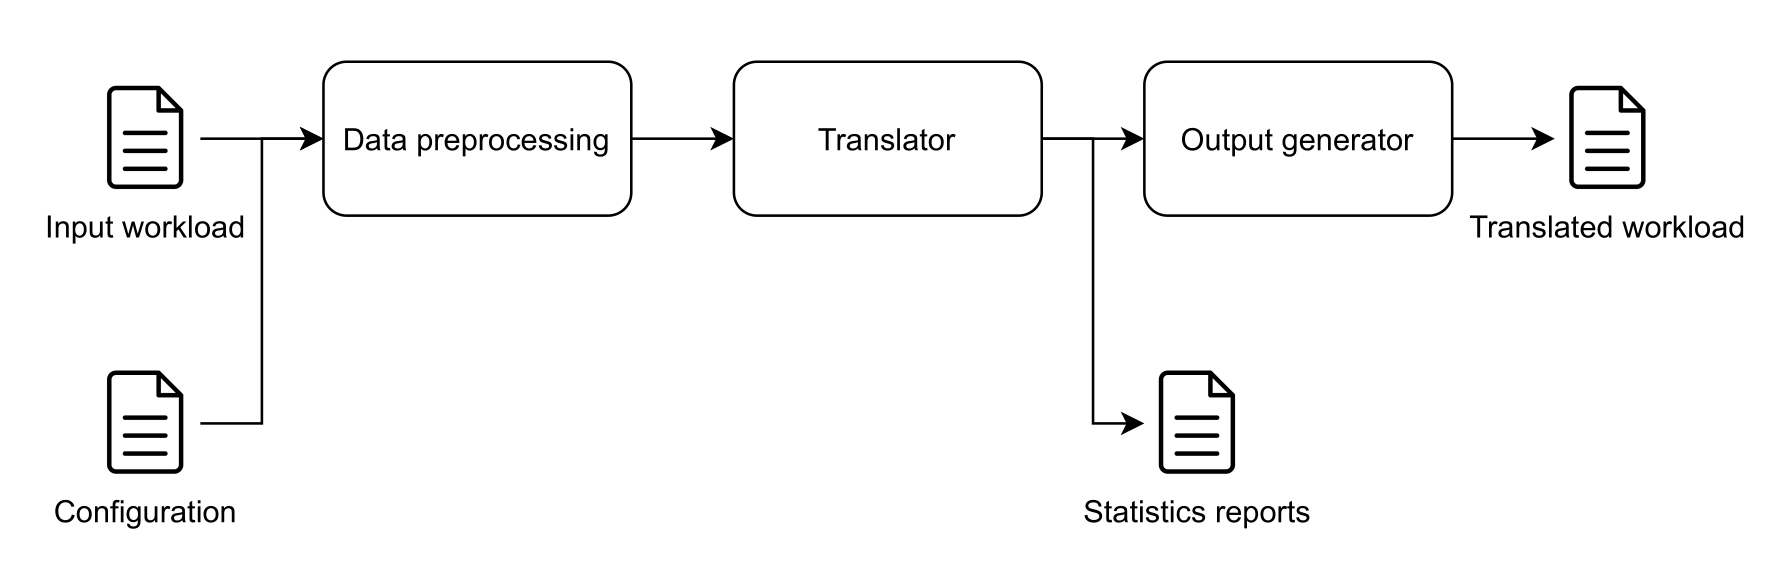
\includegraphics[width=\textwidth]{images/Parser-arq.png}
    \end{center}

\end{frame}

\begin{frame}{Generador - Tipos de cargas de trabajo} % Procesos => Trabajo realizado ???

    \centering
    \begin{table}[]
        \begin{tabular}{c c}
            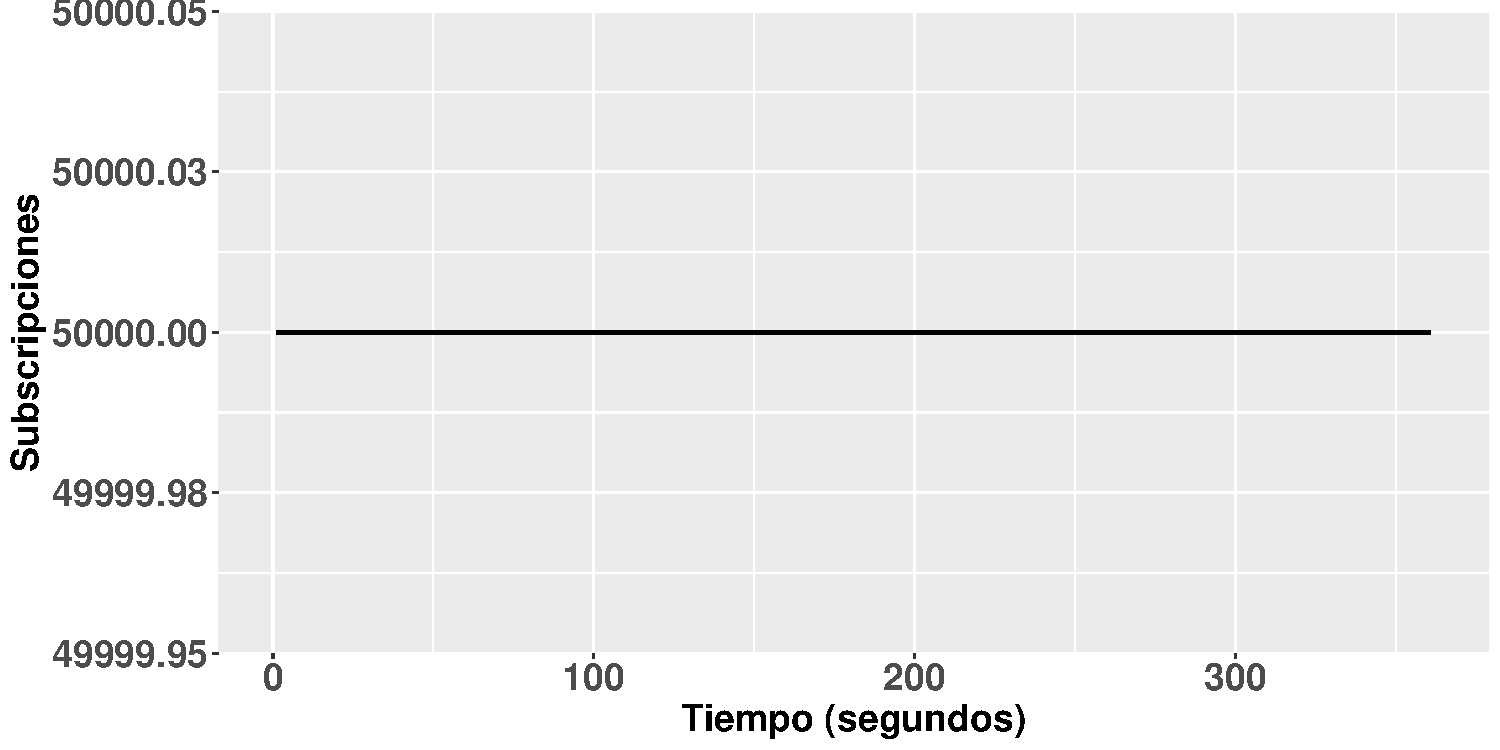
\includegraphics[width=0.45\textwidth]{images/types-of-workload/static-workload.pdf} & 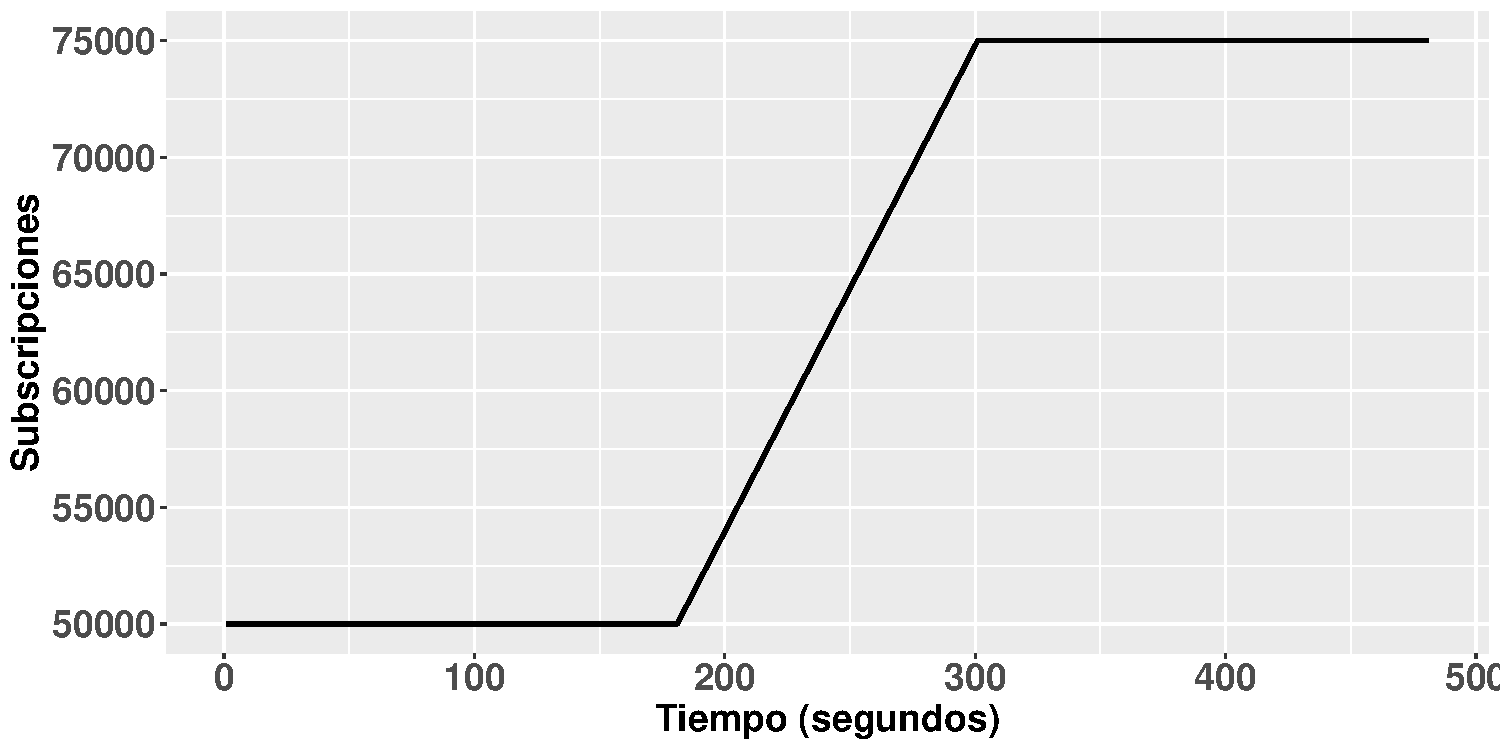
\includegraphics[width=0.45\textwidth]{images/types-of-workload/grow-workload.pdf}
        \end{tabular}
    \end{table}

    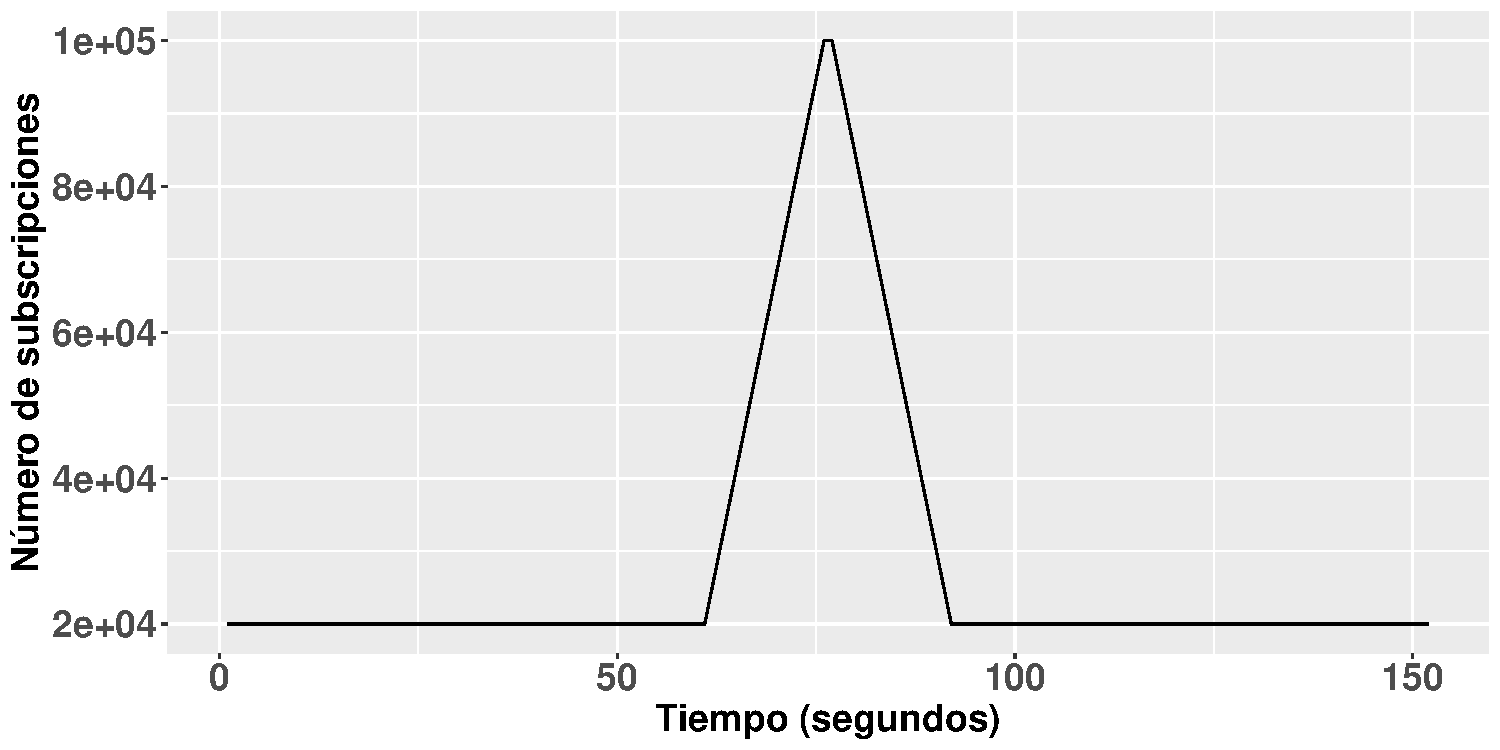
\includegraphics[width=0.5\textwidth]{images/types-of-workload/spike-workload.pdf}

\end{frame}

%%%%%%%%%%%%%%%%%%%%%%%%%%%%%%%%%%%%%%%%%%%%%%%%%%%%%%%%%%%%%%%%%%%%%%%%%%%%%%%%

\begin{frame}%{Pruebas}
    \begin{center}
        {\Large\textbf{Pruebas de rendimiento}}
    \end{center}
\end{frame}

\begin{frame}{Pruebas - Pruebas implementadas} % Procesos => Trabajo realizado ???
    
    \begin{enumerate}
        \item Toda la carga a diferentes input rates\vspace{0.25cm}
        \item Secuencia log. de subscripciones (input rate fijo)\vspace{0.25cm}
        \item Carga de subscripciones creciente (input rate fijo)\vspace{0.25cm}
        \item Carga de subscripciones estática a diferentes input rates\vspace{0.25cm}
        \item Carga de subscripciones con crecimiento puntual (input rate fijo)
    \end{enumerate}
    
        % Hablar de las pruebas que sea han realizado, relacionándolas
        % con las cargas vistas anteriormente
    
\end{frame}

\begin{frame}{Pruebas - Resultados de las pruebas} % Procesos => Trabajo realizado ???
    \begin{center}
        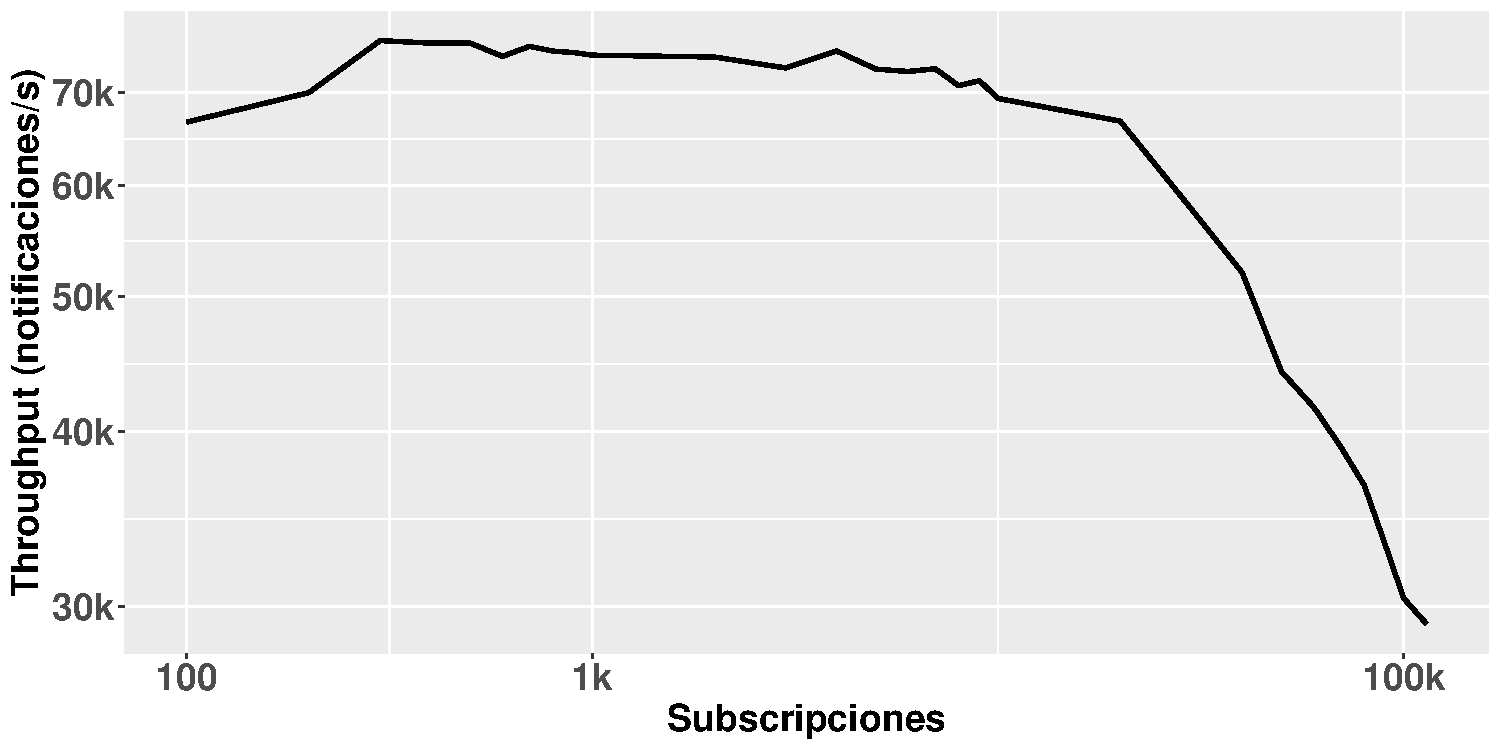
\includegraphics[width=0.8\textwidth]{images/throughput_logsubs_IR-100k.pdf}\\
        {\small Throughput de la secuencia logarítmica de subscripciones}
    \end{center}
\end{frame}

\begin{frame}{Pruebas - Resultados de las pruebas} % Procesos => Trabajo realizado ???
    \begin{center}
        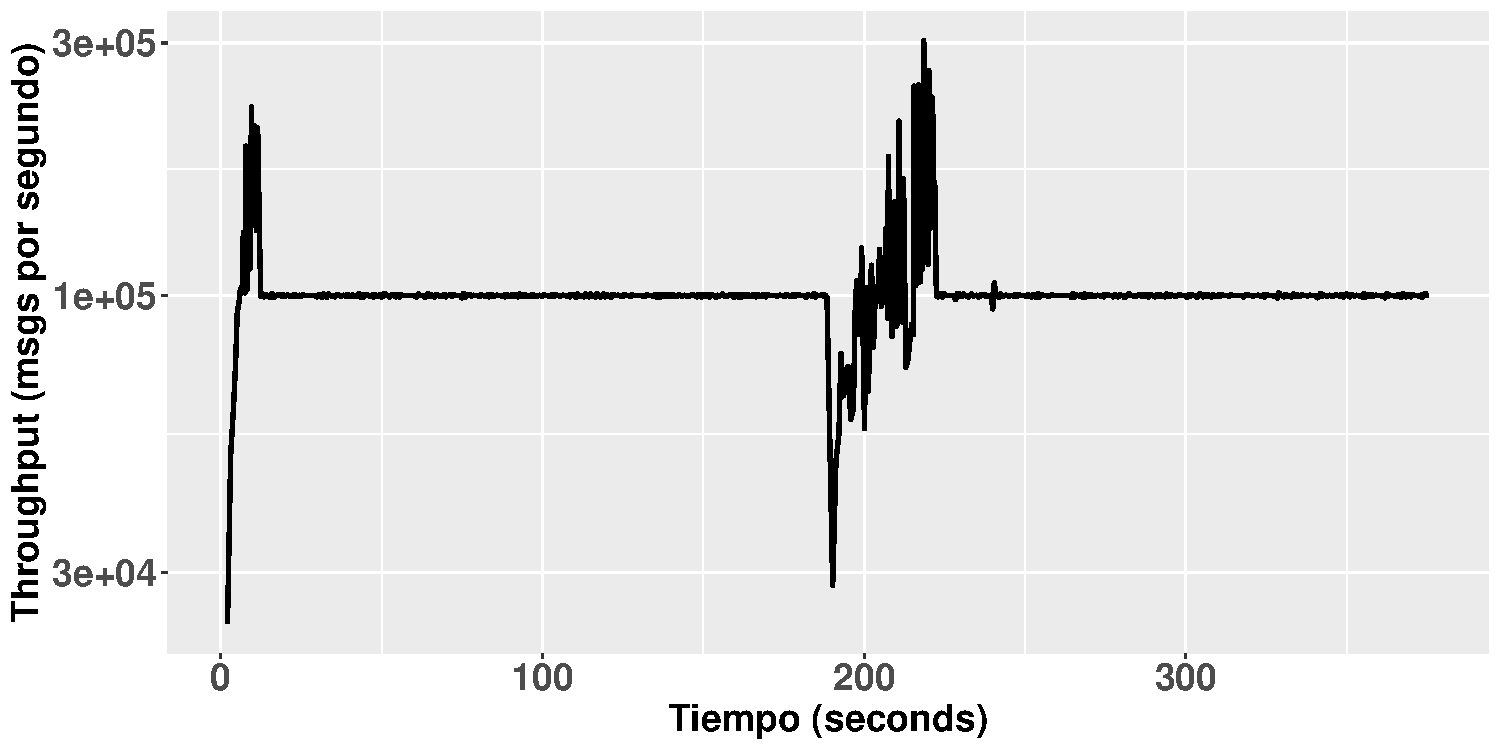
\includegraphics[width=0.8\textwidth]{images/th_test_spike_25k-113k_100000.pdf}\\
        {\small Throughput con un incremento puntual rápido del sistema}
    \end{center}
\end{frame}

%%%%%%%%%%%%%%%%%%%%%%%%%%%%%%%%%%%%%%%%%%%%%%%%%%%%%%%%%%%%%%%%%%%%%%%%%%%%%%%%

\begin{frame}%{Modelos Predictivos}
    \begin{center}
        {\Large\textbf{Implementación de los modelos predictivos}}
    \end{center}
\end{frame}

\begin{frame}{Modelos predictivos - Metodología} % Procesos => Trabajo realizado ???
    % Hablar un poco de los contenidos del script
    
    \textbf{Rolling Forecasting Origin}
    \begin{itemize}
        \item \textit{initialWindow}: tam. inicial del set de entrenamiento
        \item \textit{horizon}: tam. del set de test
        \item \textit{fixedWindow}: series de entrenamiento 
    \end{itemize}
    
    \begin{figure}
        \centering
        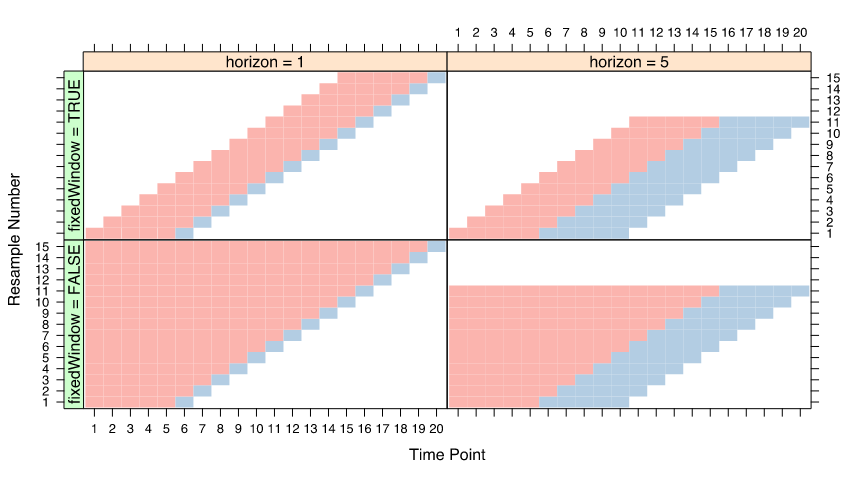
\includegraphics[width=0.75\textwidth]{images/time-series.png}
    \end{figure}
\end{frame}

\begin{frame}{Modelos predictivos - Series Temporales y ML \& DL} % Procesos => Trabajo realizado ???
    \begin{itemize}
        \item Series Temporales
        \begin{itemize}
            \item Modelos ARIMA
            \item Modelos STL con ETS\vspace{0.25cm}
        \end{itemize}
        
        \item ML \& DL
        \begin{itemize}
            \item Regresión Lineal
            \item Generalizados Aditivos
            \item Generalizados Lineales
            \item \textit{Random Forest}
            \item Redes Neuronales
        \end{itemize}
    \end{itemize}
\end{frame}

%%%%%%%%%%%%%%%%%%%%%%%%%%%%%%%%%%%%%%%%%%%%%%%%%%%%%%%%%%%%%%%%%%%%%%%%%%%%%%%%

\begin{frame}{Resultados y Conclusiones}
    \begin{itemize}
        \item Diseño e implementación de un generador que traduce cargas de trabajo entre sistemas pub/sub\vspace{0.25cm}
        \item Diseño e implementación de pruebas de rendimiento\vspace{0.25cm}
        \item Implementados modelos predictivos para predecir el rendimiento del sistema\vspace{0.75cm}

        \item Towards automatic evaluation and comparison of publish/subscribe systems performance improvements: A case study, \\ \textit{Journal of Web Engineering, JCR Q4}
    \end{itemize}
\end{frame}

%%%%%%%%%%%%%%%%%%%%%%%%%%%%%%%%%%%%%%%%%%%%%%%%%%%%%%%%%%%%%%%%%%%%%%%%%%%%%%%%

\begin{frame}{Trabajo futuro}
    \begin{itemize}
        \item Prueba y aplicación de modelos predictivos\vspace{0.5cm}
        \item Analizar la primera derivada de \textit{throughput} y \textit{tiempo de respuesta} para predecir la tendencia\vspace{0.5cm}
        \item Analizar si añadiendo más métricas de rendimiento se mejoran las predicciones\vspace{0.5cm}
        \item Aplicación de resultados al sistema de auto-escalado
    \end{itemize}
\end{frame}

%%%%%%%%%%%%%%%%%%%%%%%%%%%%%%%%%%%%%%%%%%%%%%%%%%%%%%%%%%%%%%%%%%%%%%%%%%%%%%%%

\begin{frame}%{Fin}
    \centering
    Muchas gracias por su atención.
\end{frame}

%%%%%%%%%%%%%%%%%%%%%%%%%%%%%%%%%%%%%%%%%%%%%%%%%%%%%%%%%%%%%%%%%%%%%%%%%%%%%%%%

\end{document}
